\documentclass{article}
\usepackage{fullpage,booktabs,graphicx,hyperref,float,array}
% generated by grnbench report from result files - do not edit
\newcommand{\gbCiHighAuprcRatioAutoGrnboostTwoCistargetVsGrnboostTwo}{+0.106}
\newcommand{\gbCiHighAuprcRatioAutoGrnboostTwoMotifVsGrnboostTwo}{+0.177}
\newcommand{\gbCiHighAuprcRatioAutoGrnboostTwoVsPearsonSigned}{-0.067}
\newcommand{\gbCiHighAuprcRatioAutoPearsonMotifVsMotifPrior}{+0.257}
\newcommand{\gbCiHighAuprcRatioAutoPearsonMotifVsPearsonSigned}{+0.297}
\newcommand{\gbCiHighAuprcRatioAutoRegdiffusionMotifVsRegdiffusion}{+0.308}
\newcommand{\gbCiHighAuprcRatioAutoRegdiffusionVsPearsonSigned}{+0.201}
\newcommand{\gbCiHighAuprcRatioBaselineGrnboostTwoCistargetVsGrnboostTwo}{+0.102}
\newcommand{\gbCiHighAuprcRatioBaselineGrnboostTwoMotifVsGrnboostTwo}{+0.178}
\newcommand{\gbCiHighAuprcRatioBaselineGrnboostTwoVsPearsonSigned}{-0.088}
\newcommand{\gbCiHighAuprcRatioBaselinePearsonMotifVsMotifPrior}{+0.230}
\newcommand{\gbCiHighAuprcRatioBaselinePearsonMotifVsPearsonSigned}{+0.292}
\newcommand{\gbCiHighAuprcRatioBaselineRegdiffusionMotifVsRegdiffusion}{+0.310}
\newcommand{\gbCiHighAuprcRatioBaselineRegdiffusionVsPearsonSigned}{+0.221}
\newcommand{\gbCiHighEprAutoGrnboostTwoCistargetVsGrnboostTwo}{+1.213}
\newcommand{\gbCiHighEprAutoGrnboostTwoMotifVsGrnboostTwo}{+0.837}
\newcommand{\gbCiHighEprAutoGrnboostTwoVsPearsonSigned}{-0.489}
\newcommand{\gbCiHighEprAutoPearsonMotifVsMotifPrior}{+1.002}
\newcommand{\gbCiHighEprAutoPearsonMotifVsPearsonSigned}{+0.681}
\newcommand{\gbCiHighEprAutoRegdiffusionMotifVsRegdiffusion}{+0.392}
\newcommand{\gbCiHighEprAutoRegdiffusionVsPearsonSigned}{+1.122}
\newcommand{\gbCiHighEprBaselineGrnboostTwoCistargetVsGrnboostTwo}{+1.306}
\newcommand{\gbCiHighEprBaselineGrnboostTwoMotifVsGrnboostTwo}{+0.878}
\newcommand{\gbCiHighEprBaselineGrnboostTwoVsPearsonSigned}{-0.533}
\newcommand{\gbCiHighEprBaselinePearsonMotifVsMotifPrior}{+0.909}
\newcommand{\gbCiHighEprBaselinePearsonMotifVsPearsonSigned}{+0.660}
\newcommand{\gbCiHighEprBaselineRegdiffusionMotifVsRegdiffusion}{+0.231}
\newcommand{\gbCiHighEprBaselineRegdiffusionVsPearsonSigned}{+1.255}
\newcommand{\gbCiLowAuprcRatioAutoGrnboostTwoCistargetVsGrnboostTwo}{+0.047}
\newcommand{\gbCiLowAuprcRatioAutoGrnboostTwoMotifVsGrnboostTwo}{+0.110}
\newcommand{\gbCiLowAuprcRatioAutoGrnboostTwoVsPearsonSigned}{-0.375}
\newcommand{\gbCiLowAuprcRatioAutoPearsonMotifVsMotifPrior}{-0.029}
\newcommand{\gbCiLowAuprcRatioAutoPearsonMotifVsPearsonSigned}{+0.160}
\newcommand{\gbCiLowAuprcRatioAutoRegdiffusionMotifVsRegdiffusion}{+0.136}
\newcommand{\gbCiLowAuprcRatioAutoRegdiffusionVsPearsonSigned}{+0.025}
\newcommand{\gbCiLowAuprcRatioBaselineGrnboostTwoCistargetVsGrnboostTwo}{+0.045}
\newcommand{\gbCiLowAuprcRatioBaselineGrnboostTwoMotifVsGrnboostTwo}{+0.111}
\newcommand{\gbCiLowAuprcRatioBaselineGrnboostTwoVsPearsonSigned}{-0.331}
\newcommand{\gbCiLowAuprcRatioBaselinePearsonMotifVsMotifPrior}{-0.019}
\newcommand{\gbCiLowAuprcRatioBaselinePearsonMotifVsPearsonSigned}{+0.149}
\newcommand{\gbCiLowAuprcRatioBaselineRegdiffusionMotifVsRegdiffusion}{+0.142}
\newcommand{\gbCiLowAuprcRatioBaselineRegdiffusionVsPearsonSigned}{+0.006}
\newcommand{\gbCiLowEprAutoGrnboostTwoCistargetVsGrnboostTwo}{+0.668}
\newcommand{\gbCiLowEprAutoGrnboostTwoMotifVsGrnboostTwo}{+0.511}
\newcommand{\gbCiLowEprAutoGrnboostTwoVsPearsonSigned}{-1.380}
\newcommand{\gbCiLowEprAutoPearsonMotifVsMotifPrior}{+0.294}
\newcommand{\gbCiLowEprAutoPearsonMotifVsPearsonSigned}{+0.063}
\newcommand{\gbCiLowEprAutoRegdiffusionMotifVsRegdiffusion}{-0.307}
\newcommand{\gbCiLowEprAutoRegdiffusionVsPearsonSigned}{+0.422}
\newcommand{\gbCiLowEprBaselineGrnboostTwoCistargetVsGrnboostTwo}{+0.768}
\newcommand{\gbCiLowEprBaselineGrnboostTwoMotifVsGrnboostTwo}{+0.520}
\newcommand{\gbCiLowEprBaselineGrnboostTwoVsPearsonSigned}{-1.351}
\newcommand{\gbCiLowEprBaselinePearsonMotifVsMotifPrior}{+0.263}
\newcommand{\gbCiLowEprBaselinePearsonMotifVsPearsonSigned}{+0.040}
\newcommand{\gbCiLowEprBaselineRegdiffusionMotifVsRegdiffusion}{-0.504}
\newcommand{\gbCiLowEprBaselineRegdiffusionVsPearsonSigned}{+0.543}
\newcommand{\gbDiffAuprcRatioAutoGrnboostTwoCistargetVsGrnboostTwo}{+0.076}
\newcommand{\gbDiffAuprcRatioAutoGrnboostTwoMotifVsGrnboostTwo}{+0.143}
\newcommand{\gbDiffAuprcRatioAutoGrnboostTwoVsPearsonSigned}{-0.221}
\newcommand{\gbDiffAuprcRatioAutoPearsonMotifVsMotifPrior}{+0.114}
\newcommand{\gbDiffAuprcRatioAutoPearsonMotifVsPearsonSigned}{+0.229}
\newcommand{\gbDiffAuprcRatioAutoRegdiffusionMotifVsRegdiffusion}{+0.222}
\newcommand{\gbDiffAuprcRatioAutoRegdiffusionVsPearsonSigned}{+0.113}
\newcommand{\gbDiffAuprcRatioBaselineGrnboostTwoCistargetVsGrnboostTwo}{+0.074}
\newcommand{\gbDiffAuprcRatioBaselineGrnboostTwoMotifVsGrnboostTwo}{+0.145}
\newcommand{\gbDiffAuprcRatioBaselineGrnboostTwoVsPearsonSigned}{-0.210}
\newcommand{\gbDiffAuprcRatioBaselinePearsonMotifVsMotifPrior}{+0.105}
\newcommand{\gbDiffAuprcRatioBaselinePearsonMotifVsPearsonSigned}{+0.221}
\newcommand{\gbDiffAuprcRatioBaselineRegdiffusionMotifVsRegdiffusion}{+0.226}
\newcommand{\gbDiffAuprcRatioBaselineRegdiffusionVsPearsonSigned}{+0.114}
\newcommand{\gbDiffEprAutoGrnboostTwoCistargetVsGrnboostTwo}{+0.941}
\newcommand{\gbDiffEprAutoGrnboostTwoMotifVsGrnboostTwo}{+0.674}
\newcommand{\gbDiffEprAutoGrnboostTwoVsPearsonSigned}{-0.934}
\newcommand{\gbDiffEprAutoPearsonMotifVsMotifPrior}{+0.648}
\newcommand{\gbDiffEprAutoPearsonMotifVsPearsonSigned}{+0.372}
\newcommand{\gbDiffEprAutoRegdiffusionMotifVsRegdiffusion}{+0.043}
\newcommand{\gbDiffEprAutoRegdiffusionVsPearsonSigned}{+0.772}
\newcommand{\gbDiffEprBaselineGrnboostTwoCistargetVsGrnboostTwo}{+1.037}
\newcommand{\gbDiffEprBaselineGrnboostTwoMotifVsGrnboostTwo}{+0.699}
\newcommand{\gbDiffEprBaselineGrnboostTwoVsPearsonSigned}{-0.942}
\newcommand{\gbDiffEprBaselinePearsonMotifVsMotifPrior}{+0.586}
\newcommand{\gbDiffEprBaselinePearsonMotifVsPearsonSigned}{+0.350}
\newcommand{\gbDiffEprBaselineRegdiffusionMotifVsRegdiffusion}{-0.137}
\newcommand{\gbDiffEprBaselineRegdiffusionVsPearsonSigned}{+0.899}
\newcommand{\gbFamilyAuprcRatioAuto}{14}
\newcommand{\gbFamilyAuprcRatioBaseline}{14}
\newcommand{\gbFamilyEprAuto}{14}
\newcommand{\gbFamilyEprBaseline}{14}
\newcommand{\gbMeanAuprcRatioAutoClr}{1.303}
\newcommand{\gbMeanAuprcRatioAutoGrnboostTwo}{1.098}
\newcommand{\gbMeanAuprcRatioAutoGrnboostTwoCistarget}{1.174}
\newcommand{\gbMeanAuprcRatioAutoGrnboostTwoMotif}{1.241}
\newcommand{\gbMeanAuprcRatioAutoMotifPrior}{1.433}
\newcommand{\gbMeanAuprcRatioAutoPearsonMotif}{1.547}
\newcommand{\gbMeanAuprcRatioAutoPearsonSigned}{1.319}
\newcommand{\gbMeanAuprcRatioAutoRegdiffusion}{1.432}
\newcommand{\gbMeanAuprcRatioAutoRegdiffusionMotif}{1.654}
\newcommand{\gbMeanAuprcRatioAutoSpearmanSigned}{1.358}
\newcommand{\gbNAuprcRatioAutoGrnboostTwoCistargetVsGrnboostTwo}{12}
\newcommand{\gbNAuprcRatioAutoGrnboostTwoMotifVsGrnboostTwo}{12}
\newcommand{\gbNAuprcRatioAutoGrnboostTwoVsPearsonSigned}{12}
\newcommand{\gbNAuprcRatioAutoPearsonMotifVsMotifPrior}{12}
\newcommand{\gbNAuprcRatioAutoPearsonMotifVsPearsonSigned}{12}
\newcommand{\gbNAuprcRatioAutoRegdiffusionMotifVsRegdiffusion}{12}
\newcommand{\gbNAuprcRatioAutoRegdiffusionVsPearsonSigned}{12}
\newcommand{\gbNAuprcRatioBaselineGrnboostTwoCistargetVsGrnboostTwo}{12}
\newcommand{\gbNAuprcRatioBaselineGrnboostTwoMotifVsGrnboostTwo}{12}
\newcommand{\gbNAuprcRatioBaselineGrnboostTwoVsPearsonSigned}{12}
\newcommand{\gbNAuprcRatioBaselinePearsonMotifVsMotifPrior}{12}
\newcommand{\gbNAuprcRatioBaselinePearsonMotifVsPearsonSigned}{12}
\newcommand{\gbNAuprcRatioBaselineRegdiffusionMotifVsRegdiffusion}{12}
\newcommand{\gbNAuprcRatioBaselineRegdiffusionVsPearsonSigned}{12}
\newcommand{\gbNAutoClr}{12}
\newcommand{\gbNAutoGrnboostTwo}{12}
\newcommand{\gbNAutoGrnboostTwoCistarget}{12}
\newcommand{\gbNAutoGrnboostTwoMotif}{12}
\newcommand{\gbNAutoMotifPrior}{12}
\newcommand{\gbNAutoPearsonMotif}{12}
\newcommand{\gbNAutoPearsonSigned}{12}
\newcommand{\gbNAutoRegdiffusion}{12}
\newcommand{\gbNAutoRegdiffusionMotif}{12}
\newcommand{\gbNAutoSpearmanSigned}{12}
\newcommand{\gbNDatasets}{12}
\newcommand{\gbNEprAutoGrnboostTwoCistargetVsGrnboostTwo}{12}
\newcommand{\gbNEprAutoGrnboostTwoMotifVsGrnboostTwo}{12}
\newcommand{\gbNEprAutoGrnboostTwoVsPearsonSigned}{12}
\newcommand{\gbNEprAutoPearsonMotifVsMotifPrior}{12}
\newcommand{\gbNEprAutoPearsonMotifVsPearsonSigned}{12}
\newcommand{\gbNEprAutoRegdiffusionMotifVsRegdiffusion}{12}
\newcommand{\gbNEprAutoRegdiffusionVsPearsonSigned}{12}
\newcommand{\gbNEprBaselineGrnboostTwoCistargetVsGrnboostTwo}{12}
\newcommand{\gbNEprBaselineGrnboostTwoMotifVsGrnboostTwo}{12}
\newcommand{\gbNEprBaselineGrnboostTwoVsPearsonSigned}{12}
\newcommand{\gbNEprBaselinePearsonMotifVsMotifPrior}{12}
\newcommand{\gbNEprBaselinePearsonMotifVsPearsonSigned}{12}
\newcommand{\gbNEprBaselineRegdiffusionMotifVsRegdiffusion}{12}
\newcommand{\gbNEprBaselineRegdiffusionVsPearsonSigned}{12}
\newcommand{\gbPHolmAuprcRatioAutoGrnboostTwoCistargetVsGrnboostTwo}{0.00085}
\newcommand{\gbPHolmAuprcRatioAutoGrnboostTwoMotifVsGrnboostTwo}{9.6e-06}
\newcommand{\gbPHolmAuprcRatioAutoGrnboostTwoVsPearsonSigned}{1.000}
\newcommand{\gbPHolmAuprcRatioAutoPearsonMotifVsMotifPrior}{0.429}
\newcommand{\gbPHolmAuprcRatioAutoPearsonMotifVsPearsonSigned}{9.9e-05}
\newcommand{\gbPHolmAuprcRatioAutoRegdiffusionMotifVsRegdiffusion}{0.00085}
\newcommand{\gbPHolmAuprcRatioAutoRegdiffusionVsPearsonSigned}{0.074}
\newcommand{\gbPHolmAuprcRatioBaselineGrnboostTwoCistargetVsGrnboostTwo}{0.00074}
\newcommand{\gbPHolmAuprcRatioBaselineGrnboostTwoMotifVsGrnboostTwo}{8.3e-06}
\newcommand{\gbPHolmAuprcRatioBaselineGrnboostTwoVsPearsonSigned}{1.000}
\newcommand{\gbPHolmAuprcRatioBaselinePearsonMotifVsMotifPrior}{0.356}
\newcommand{\gbPHolmAuprcRatioBaselinePearsonMotifVsPearsonSigned}{0.0002}
\newcommand{\gbPHolmAuprcRatioBaselineRegdiffusionMotifVsRegdiffusion}{0.00061}
\newcommand{\gbPHolmAuprcRatioBaselineRegdiffusionVsPearsonSigned}{0.179}
\newcommand{\gbPHolmEprAutoGrnboostTwoCistargetVsGrnboostTwo}{6.9e-05}
\newcommand{\gbPHolmEprAutoGrnboostTwoMotifVsGrnboostTwo}{1.3e-05}
\newcommand{\gbPHolmEprAutoGrnboostTwoVsPearsonSigned}{1.000}
\newcommand{\gbPHolmEprAutoPearsonMotifVsMotifPrior}{0.010}
\newcommand{\gbPHolmEprAutoPearsonMotifVsPearsonSigned}{0.101}
\newcommand{\gbPHolmEprAutoRegdiffusionMotifVsRegdiffusion}{1.000}
\newcommand{\gbPHolmEprAutoRegdiffusionVsPearsonSigned}{0.003}
\newcommand{\gbPHolmEprBaselineGrnboostTwoCistargetVsGrnboostTwo}{2.4e-05}
\newcommand{\gbPHolmEprBaselineGrnboostTwoMotifVsGrnboostTwo}{2.3e-05}
\newcommand{\gbPHolmEprBaselineGrnboostTwoVsPearsonSigned}{1.000}
\newcommand{\gbPHolmEprBaselinePearsonMotifVsMotifPrior}{0.011}
\newcommand{\gbPHolmEprBaselinePearsonMotifVsPearsonSigned}{0.137}
\newcommand{\gbPHolmEprBaselineRegdiffusionMotifVsRegdiffusion}{1.000}
\newcommand{\gbPHolmEprBaselineRegdiffusionVsPearsonSigned}{0.001}
\newcommand{\gbPHolmRevAuprcRatioAutoGrnboostTwoCistargetVsGrnboostTwo}{1.000}
\newcommand{\gbPHolmRevAuprcRatioAutoGrnboostTwoMotifVsGrnboostTwo}{1.000}
\newcommand{\gbPHolmRevAuprcRatioAutoGrnboostTwoVsPearsonSigned}{0.046}
\newcommand{\gbPHolmRevAuprcRatioAutoPearsonMotifVsMotifPrior}{1.000}
\newcommand{\gbPHolmRevAuprcRatioAutoPearsonMotifVsPearsonSigned}{1.000}
\newcommand{\gbPHolmRevAuprcRatioAutoRegdiffusionMotifVsRegdiffusion}{1.000}
\newcommand{\gbPHolmRevAuprcRatioAutoRegdiffusionVsPearsonSigned}{1.000}
\newcommand{\gbPHolmRevAuprcRatioBaselineGrnboostTwoCistargetVsGrnboostTwo}{1.000}
\newcommand{\gbPHolmRevAuprcRatioBaselineGrnboostTwoMotifVsGrnboostTwo}{1.000}
\newcommand{\gbPHolmRevAuprcRatioBaselineGrnboostTwoVsPearsonSigned}{0.015}
\newcommand{\gbPHolmRevAuprcRatioBaselinePearsonMotifVsMotifPrior}{1.000}
\newcommand{\gbPHolmRevAuprcRatioBaselinePearsonMotifVsPearsonSigned}{1.000}
\newcommand{\gbPHolmRevAuprcRatioBaselineRegdiffusionMotifVsRegdiffusion}{1.000}
\newcommand{\gbPHolmRevAuprcRatioBaselineRegdiffusionVsPearsonSigned}{1.000}
\newcommand{\gbPHolmRevEprAutoGrnboostTwoCistargetVsGrnboostTwo}{1.000}
\newcommand{\gbPHolmRevEprAutoGrnboostTwoMotifVsGrnboostTwo}{1.000}
\newcommand{\gbPHolmRevEprAutoGrnboostTwoVsPearsonSigned}{0.004}
\newcommand{\gbPHolmRevEprAutoPearsonMotifVsMotifPrior}{1.000}
\newcommand{\gbPHolmRevEprAutoPearsonMotifVsPearsonSigned}{1.000}
\newcommand{\gbPHolmRevEprAutoRegdiffusionMotifVsRegdiffusion}{1.000}
\newcommand{\gbPHolmRevEprAutoRegdiffusionVsPearsonSigned}{1.000}
\newcommand{\gbPHolmRevEprBaselineGrnboostTwoCistargetVsGrnboostTwo}{1.000}
\newcommand{\gbPHolmRevEprBaselineGrnboostTwoMotifVsGrnboostTwo}{1.000}
\newcommand{\gbPHolmRevEprBaselineGrnboostTwoVsPearsonSigned}{0.002}
\newcommand{\gbPHolmRevEprBaselinePearsonMotifVsMotifPrior}{1.000}
\newcommand{\gbPHolmRevEprBaselinePearsonMotifVsPearsonSigned}{1.000}
\newcommand{\gbPHolmRevEprBaselineRegdiffusionMotifVsRegdiffusion}{1.000}
\newcommand{\gbPHolmRevEprBaselineRegdiffusionVsPearsonSigned}{1.000}

\title{EXP-20260925-LM-1: Does a motif (sequence) prior lift GRN recovery on real data?}
\author{grnbench report generated from EXP-20260925-LM-1}
\date{}
\begin{document}
\maketitle
\section*{Status}
Experiment EXP-20260925-LM-1, type: exploratory.. Record status: done. Reproduced by: nobody yet.
\section{Configuration summary}
\begin{table}[H]\centering\small
\caption{Configuration of the run, from the experiment record and the run folder.}
\begin{tabular}{p{0.3\linewidth}p{0.62\linewidth}}\toprule
experiment & EXP-20260925-LM-1 \\
type & exploratory. The comparison family was declared in code (real\_bench.DECLARED\_PAIRS) before the run, but there was no committed registration record. Needs a confirmatory rerun before it feeds a headline claim. \\
owner & LM (agent run on Luca's laptop) \\
datasets (rows) & 12 \\
models & clr, grnboost2, grnboost2\_cistarget, grnboost2\_motif, motif\_prior, pearson\_motif, pearson\_signed, regdiffusion, regdiffusion\_motif, spearman\_signed \\
arms & auto, baseline \\
code & commit 942cdea of Luca's offline history (its tree is part of the first commit of this repo); CODE\_COMMIT in the results folder \\
code commit (run folder) & 942cdea61936cbc96bac0a83c344e5cd03f94bcd \\
environment & Python 3.11.9 (Windows), requirements/lock-py311.txt + regdiffusion 0.2.3, torch 2.14.0 CPU \\
machine & local laptop, 3 workers, 03:28-05:18, 13 datasets, 0 errors \\
seeds & reference split seed 0; at most 3,000 cells per context \\
run folder & benchmarks/results/engine-2026-09-25-models/test12 \\
generated & 2026-09-25 18:40 \\
\bottomrule\end{tabular}\end{table}

\section{Methods}
\begin{description}
\item[type] exploratory. The comparison family was declared in code (real\_bench.DECLARED\_PAIRS) before the run, but there was no committed registration record. Needs a confirmatory rerun before it feeds a headline claim.
\item[hypothesis] combining a cisTarget motif prior with a co-expression model improves recovery of CollecTRI targets on real scRNA-seq.
\item[primary endpoint] AUPRC ratio on the CollecTRI evaluation half (selection half used only to choose the pipeline, screen.split\_reference, seed 0); secondary: EPR
\item[unit of analysis] dataset, n = 12 (CELLxGENE, 8 protocols, human 7 + mouse 5)
\item[exclusions] PBMC3k (used for development; reported separately as n = 13); a BD Rhapsody 460-gene targeted panel (not a transcriptome), removed from tasks.json before the run
\item[comparison family] 7 pairs x 2 directions per metric and arm (real\_bench.DECLARED\_PAIRS), paired t, Holm
\item[seeds] reference split seed 0; at most 3,000 cells per context
\item[code] commit 942cdea of Luca's offline history (its tree is part of the first commit of this repo); CODE\_COMMIT in the results folder
\item[environment] Python 3.11.9 (Windows), requirements/lock-py311.txt + regdiffusion 0.2.3, torch 2.14.0 CPU
\item[data] experiments/datasets.tsv (cellxgene/*, 10x\_pbmc3k/filtered, references/collectri\_*, cistarget/*)
\item[machine] local laptop, 3 workers, 03:28-05:18, 13 datasets, 0 errors
\item[models scored] clr, grnboost2, grnboost2\_cistarget, grnboost2\_motif, motif\_prior, pearson\_motif, pearson\_signed, regdiffusion, regdiffusion\_motif, spearman\_signed
\end{description}

\section{Results}
\subsection{Primary comparison}
\paragraph{Primary comparison (exploratory).} pearson\_motif $>$ pearson\_signed on AUPRC ratio, auto pipeline. Mean paired difference \gbDiffAuprcRatioAutoPearsonMotifVsPearsonSigned{} (95\% interval \gbCiLowAuprcRatioAutoPearsonMotifVsPearsonSigned{} to \gbCiHighAuprcRatioAutoPearsonMotifVsPearsonSigned{}), n = \gbNAuprcRatioAutoPearsonMotifVsPearsonSigned{} datasets, paired t, Holm over \gbFamilyAuprcRatioAuto{} directed hypotheses: $p_{\mathrm{Holm}}$ = \gbPHolmAuprcRatioAutoPearsonMotifVsPearsonSigned{}. Verdict by the rule fixed in the record: \textbf{supported}. Exploratory: this cannot support a headline claim.

\subsection{Performance per model, across datasets}
\begin{table}[H]\centering\small
\caption{Reference recovery per model (CollecTRI evaluation half; AUPRC ratio, 1 = random). Unit = dataset; n per model shown.}
\begin{tabular}{lrrrr}\toprule
model & n & mean (auto) & median (auto) & mean (baseline) \\ \midrule
regdiffusion\_motif & 12 & 1.654 & 1.624 & 1.657 \\
pearson\_motif & 12 & 1.547 & 1.499 & 1.538 \\
motif\_prior & 12 & 1.433 & 1.437 & 1.432 \\
regdiffusion & 12 & 1.432 & 1.375 & 1.430 \\
spearman\_signed & 12 & 1.358 & 1.358 & 1.355 \\
pearson\_signed & 12 & 1.319 & 1.279 & 1.317 \\
clr & 12 & 1.303 & 1.283 & 1.310 \\
grnboost2\_motif & 12 & 1.241 & 1.216 & 1.252 \\
grnboost2\_cistarget & 12 & 1.174 & 1.171 & 1.181 \\
grnboost2 & 12 & 1.098 & 1.098 & 1.107 \\
\bottomrule\end{tabular}\end{table}

\subsection{Performance per dataset}
\begin{table}[H]\centering\scriptsize
\caption{AUPRC ratio per dataset, auto pipeline (1 = random); the unit of analysis.}
\resizebox{\linewidth}{!}{\begin{tabular}{lrrrrrrrrrr}\toprule
dataset & regdiffusion\_motif & pearson\_motif & motif\_prior & regdiffusion & spearman\_signed & pearson\_signed & clr & grnboost2\_motif & grnboost2\_cistarget & grnboost2 \\ \midrule
10x-3-v2\_\_homo-sapiens\_\_superior-frontal-gyrus\_\_ & 1.63 & 1.48 & 1.54 & 1.27 & 1.27 & 1.14 & 1.15 & 1.19 & 1.10 & 1.04 \\
10x-3-v2\_\_mus-musculus\_\_large-intestine\_\_de4e7a0 & 1.67 & 1.45 & 1.28 & 1.54 & 1.43 & 1.26 & 1.40 & 1.22 & 1.19 & 1.10 \\
10x-3-v3\_\_homo-sapiens\_\_liver\_\_d7476ae2 & 2.07 & 2.05 & 1.44 & 1.94 & 1.94 & 1.97 & 1.62 & 1.18 & 1.12 & 1.07 \\
10x-3-v3\_\_mus-musculus\_\_cervical-spinal-cord\_\_9f & 1.62 & 1.36 & 1.64 & 1.20 & 1.05 & 0.97 & 1.23 & 1.29 & 1.14 & 1.10 \\
10x-5-v1\_\_homo-sapiens\_\_lung\_\_703f00e6 & 1.62 & 1.39 & 1.26 & 1.65 & 1.44 & 1.30 & 1.45 & 1.21 & 1.26 & 1.11 \\
10x-5-v2\_\_mus-musculus\_\_caecum\_\_0a1ad9d5 & 1.71 & 1.68 & 1.64 & 1.30 & 1.30 & 1.30 & 1.26 & 1.40 & 1.28 & 1.13 \\
10x-multiome\_\_homo-sapiens\_\_atrioventricular-nod & 1.71 & 1.52 & 1.50 & 1.47 & 1.58 & 1.25 & 1.30 & 1.21 & 1.10 & 1.06 \\
cel-seq2\_\_homo-sapiens\_\_left-main-bronchus\_\_03da & 1.58 & 1.61 & 1.36 & 1.40 & 1.41 & 1.40 & 1.26 & 1.22 & 1.21 & 1.10 \\
cel-seq\_\_homo-sapiens\_\_epithelium-of-main-bronch & 1.58 & 1.41 & 1.43 & 1.35 & 1.17 & 1.16 & 1.32 & 1.21 & 1.17 & 1.05 \\
patch-seq\_\_mus-musculus\_\_primary-motor-cortex\_\_8 & 1.43 & 1.37 & 1.27 & 1.31 & 1.16 & 1.22 & 1.14 & 1.20 & 1.17 & 1.14 \\
smart-seq2\_\_homo-sapiens\_\_blood\_\_a5d95a42 & 1.63 & 1.59 & 1.53 & 1.30 & 1.11 & 1.30 & 1.14 & 1.22 & 1.12 & 1.08 \\
smart-seq2\_\_mus-musculus\_\_aorta\_\_0380ddce & 1.62 & 1.67 & 1.30 & 1.45 & 1.43 & 1.55 & 1.37 & 1.33 & 1.23 & 1.20 \\
\midrule
mean & 1.65 & 1.55 & 1.43 & 1.43 & 1.36 & 1.32 & 1.30 & 1.24 & 1.17 & 1.10 \\
median & 1.62 & 1.50 & 1.44 & 1.38 & 1.36 & 1.28 & 1.28 & 1.22 & 1.17 & 1.10 \\
SD & 0.15 & 0.20 & 0.14 & 0.20 & 0.24 & 0.25 & 0.14 & 0.07 & 0.06 & 0.04 \\
\bottomrule\end{tabular}}\end{table}

\subsection{Comparative summary: declared comparisons}
\begin{table}[H]\centering\small
\caption{Declared comparisons, AUPRC ratio, auto pipeline: paired t over datasets (compare\_units), two-sided per direction, Holm over 14 directed hypotheses; 95\% interval of the mean paired difference.}
\begin{tabular}{llrrlrrl}\toprule
A & B & n & mean A$-$B & 95\% interval & $p_{A>B}$ Holm & $p_{B>A}$ Holm & supported \\ \midrule
pearson\_motif & pearson\_signed & 12 & +0.229 & [+0.160, +0.297] & 9.9e-05 & 1.000 & pearson\_motif \\
grnboost2\_motif & grnboost2 & 12 & +0.143 & [+0.110, +0.177] & 9.6e-06 & 1.000 & grnboost2\_motif \\
regdiffusion\_motif & regdiffusion & 12 & +0.222 & [+0.136, +0.308] & 0.00085 & 1.000 & regdiffusion\_motif \\
grnboost2\_cistarget & grnboost2 & 12 & +0.076 & [+0.047, +0.106] & 0.00085 & 1.000 & grnboost2\_cistarget \\
pearson\_motif & motif\_prior & 12 & +0.114 & [-0.029, +0.257] & 0.429 & 1.000 & unresolved \\
grnboost2 & pearson\_signed & 12 & -0.221 & [-0.375, -0.067] & 1.000 & 0.046 & pearson\_signed \\
regdiffusion & pearson\_signed & 12 & +0.113 & [+0.025, +0.201] & 0.074 & 1.000 & unresolved \\
\bottomrule\end{tabular}\end{table}

\begin{table}[H]\centering\small
\caption{Declared comparisons, AUPRC ratio, baseline pipeline: paired t over datasets (compare\_units), two-sided per direction, Holm over 14 directed hypotheses; 95\% interval of the mean paired difference.}
\begin{tabular}{llrrlrrl}\toprule
A & B & n & mean A$-$B & 95\% interval & $p_{A>B}$ Holm & $p_{B>A}$ Holm & supported \\ \midrule
pearson\_motif & pearson\_signed & 12 & +0.221 & [+0.149, +0.292] & 0.0002 & 1.000 & pearson\_motif \\
grnboost2\_motif & grnboost2 & 12 & +0.145 & [+0.111, +0.178] & 8.3e-06 & 1.000 & grnboost2\_motif \\
regdiffusion\_motif & regdiffusion & 12 & +0.226 & [+0.142, +0.310] & 0.00061 & 1.000 & regdiffusion\_motif \\
grnboost2\_cistarget & grnboost2 & 12 & +0.074 & [+0.045, +0.102] & 0.00074 & 1.000 & grnboost2\_cistarget \\
pearson\_motif & motif\_prior & 12 & +0.105 & [-0.019, +0.230] & 0.356 & 1.000 & unresolved \\
grnboost2 & pearson\_signed & 12 & -0.210 & [-0.331, -0.088] & 1.000 & 0.015 & pearson\_signed \\
regdiffusion & pearson\_signed & 12 & +0.114 & [+0.006, +0.221] & 0.179 & 1.000 & unresolved \\
\bottomrule\end{tabular}\end{table}

\begin{table}[H]\centering\small
\caption{Declared comparisons, EPR, auto pipeline: paired t over datasets (compare\_units), two-sided per direction, Holm over 14 directed hypotheses; 95\% interval of the mean paired difference.}
\begin{tabular}{llrrlrrl}\toprule
A & B & n & mean A$-$B & 95\% interval & $p_{A>B}$ Holm & $p_{B>A}$ Holm & supported \\ \midrule
pearson\_motif & pearson\_signed & 12 & +0.372 & [+0.063, +0.681] & 0.101 & 1.000 & unresolved \\
grnboost2\_motif & grnboost2 & 12 & +0.674 & [+0.511, +0.837] & 1.3e-05 & 1.000 & grnboost2\_motif \\
regdiffusion\_motif & regdiffusion & 12 & +0.043 & [-0.307, +0.392] & 1.000 & 1.000 & unresolved \\
grnboost2\_cistarget & grnboost2 & 12 & +0.941 & [+0.668, +1.213] & 6.9e-05 & 1.000 & grnboost2\_cistarget \\
pearson\_motif & motif\_prior & 12 & +0.648 & [+0.294, +1.002] & 0.010 & 1.000 & pearson\_motif \\
grnboost2 & pearson\_signed & 12 & -0.934 & [-1.380, -0.489] & 1.000 & 0.004 & pearson\_signed \\
regdiffusion & pearson\_signed & 12 & +0.772 & [+0.422, +1.122] & 0.003 & 1.000 & regdiffusion \\
\bottomrule\end{tabular}\end{table}

\begin{table}[H]\centering\small
\caption{Declared comparisons, EPR, baseline pipeline: paired t over datasets (compare\_units), two-sided per direction, Holm over 14 directed hypotheses; 95\% interval of the mean paired difference.}
\begin{tabular}{llrrlrrl}\toprule
A & B & n & mean A$-$B & 95\% interval & $p_{A>B}$ Holm & $p_{B>A}$ Holm & supported \\ \midrule
pearson\_motif & pearson\_signed & 12 & +0.350 & [+0.040, +0.660] & 0.137 & 1.000 & unresolved \\
grnboost2\_motif & grnboost2 & 12 & +0.699 & [+0.520, +0.878] & 2.3e-05 & 1.000 & grnboost2\_motif \\
regdiffusion\_motif & regdiffusion & 12 & -0.137 & [-0.504, +0.231] & 1.000 & 1.000 & unresolved \\
grnboost2\_cistarget & grnboost2 & 12 & +1.037 & [+0.768, +1.306] & 2.4e-05 & 1.000 & grnboost2\_cistarget \\
pearson\_motif & motif\_prior & 12 & +0.586 & [+0.263, +0.909] & 0.011 & 1.000 & pearson\_motif \\
grnboost2 & pearson\_signed & 12 & -0.942 & [-1.351, -0.533] & 1.000 & 0.002 & pearson\_signed \\
regdiffusion & pearson\_signed & 12 & +0.899 & [+0.543, +1.255] & 0.001 & 1.000 & regdiffusion \\
\bottomrule\end{tabular}\end{table}

\section{Visualizations and explainability}
\begin{figure}[H]\centering
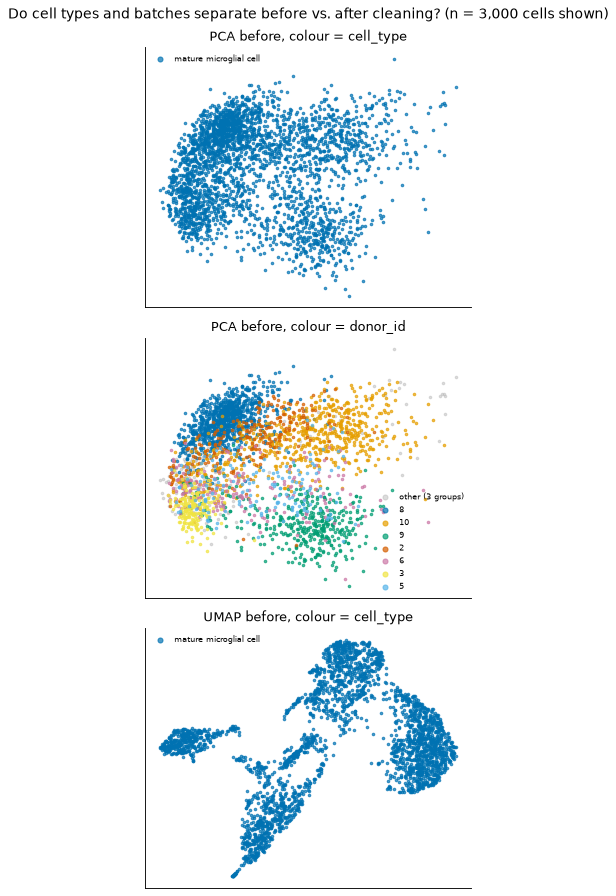
\includegraphics[width=0.85\linewidth]{../viz/embed_cxg__10x-3-v2__homo-sapiens__superior-frontal-gyrus__bdacc907.png}
\caption{-   (n = 3799 cells) - built from  tasks.json (raw data)}
\end{figure}
\begin{figure}[H]\centering
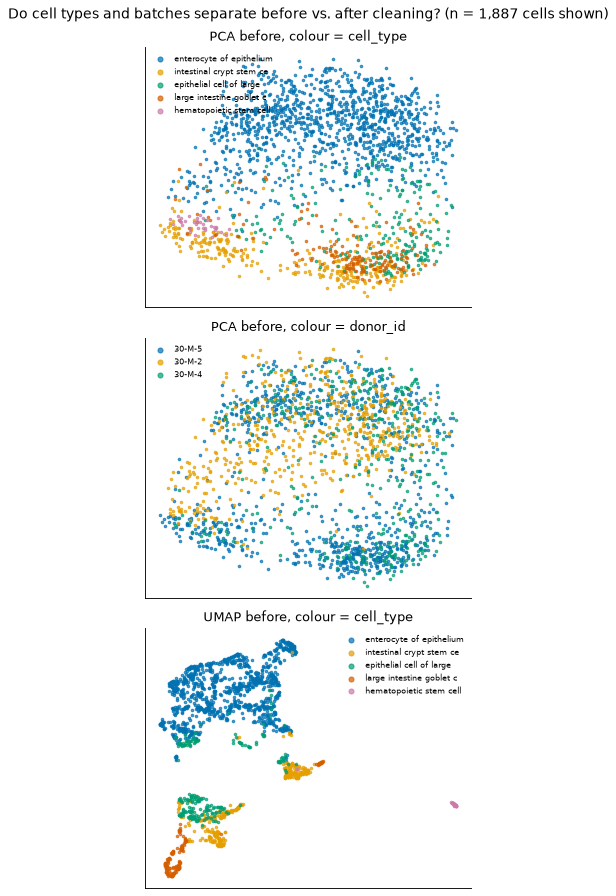
\includegraphics[width=0.85\linewidth]{../viz/embed_cxg__10x-3-v2__mus-musculus__large-intestine__de4e7a0c.png}
\caption{-   (n = 1887 cells) - built from  tasks.json (raw data)}
\end{figure}
\begin{figure}[H]\centering
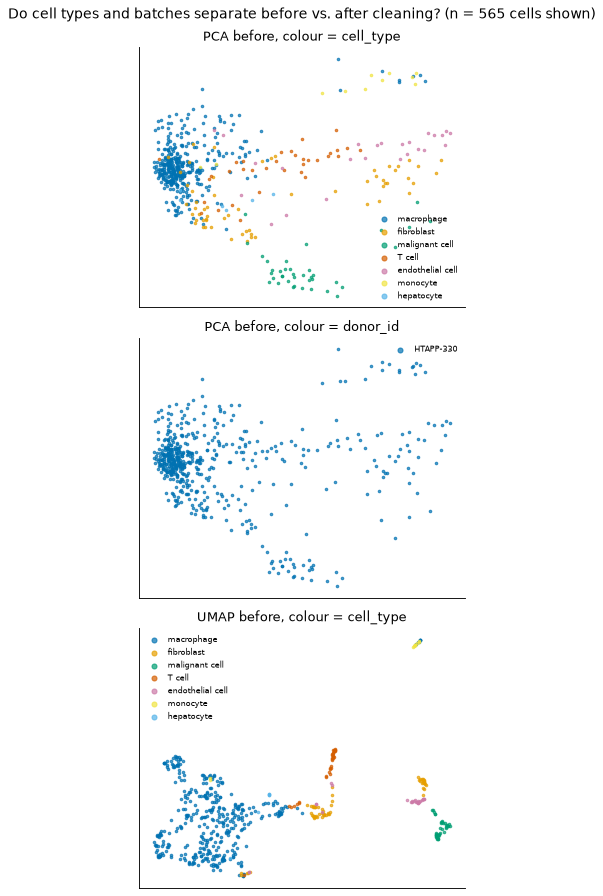
\includegraphics[width=0.85\linewidth]{../viz/embed_cxg__10x-3-v3__homo-sapiens__liver__d7476ae2.png}
\caption{-   (n = 565 cells) - built from  tasks.json (raw data)}
\end{figure}
\begin{figure}[H]\centering
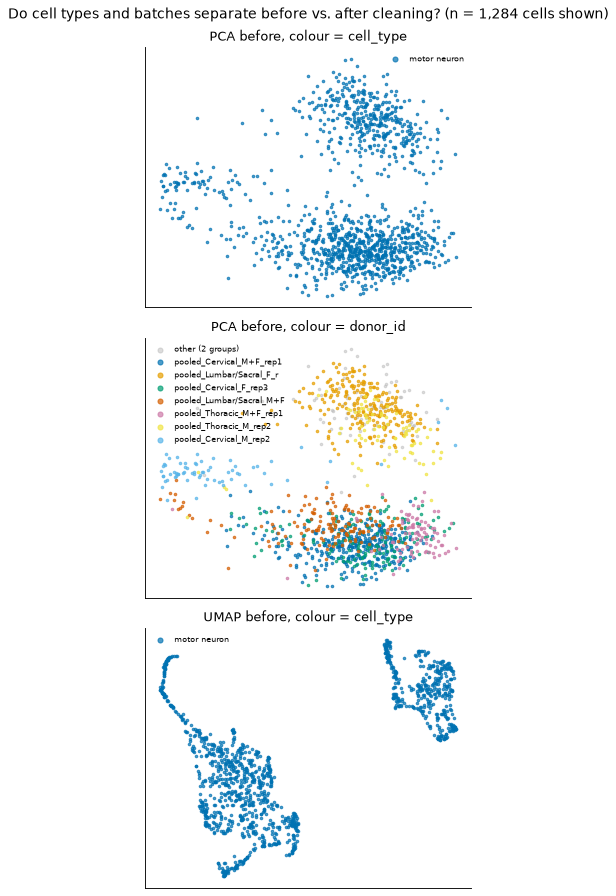
\includegraphics[width=0.85\linewidth]{../viz/embed_cxg__10x-3-v3__mus-musculus__cervical-spinal-cord__9fcd3812.png}
\caption{-   (n = 1284 cells) - built from  tasks.json (raw data)}
\end{figure}
\begin{figure}[H]\centering
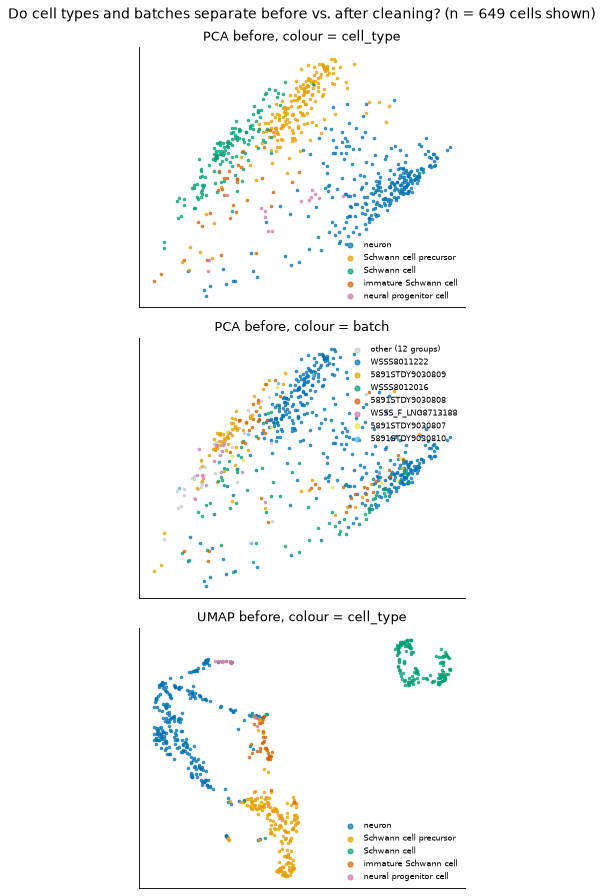
\includegraphics[width=0.85\linewidth]{../viz/embed_cxg__10x-5-v1__homo-sapiens__lung__703f00e6.png}
\caption{-   (n = 649 cells) - built from  tasks.json (raw data)}
\end{figure}
\begin{figure}[H]\centering
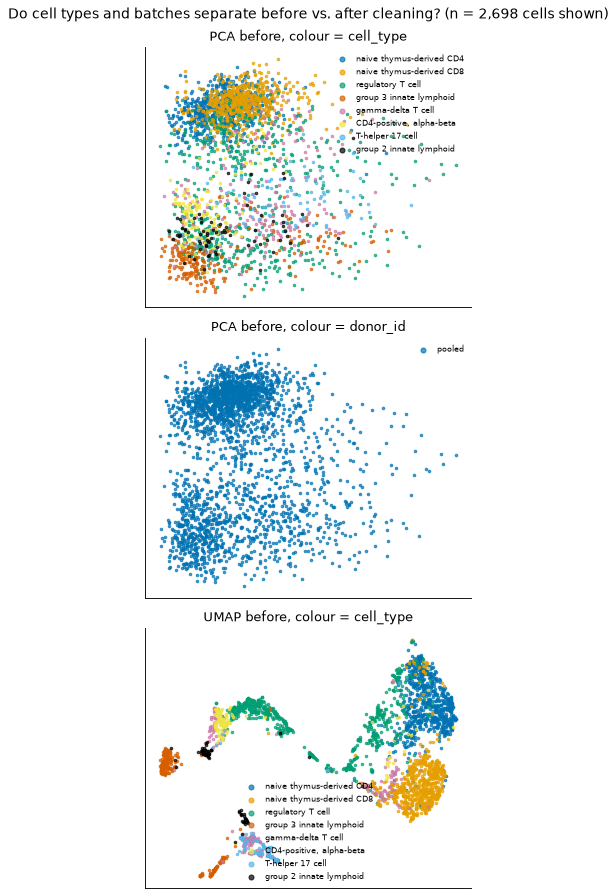
\includegraphics[width=0.85\linewidth]{../viz/embed_cxg__10x-5-v2__mus-musculus__caecum__0a1ad9d5.png}
\caption{-   (n = 2698 cells) - built from  tasks.json (raw data)}
\end{figure}
\begin{figure}[H]\centering
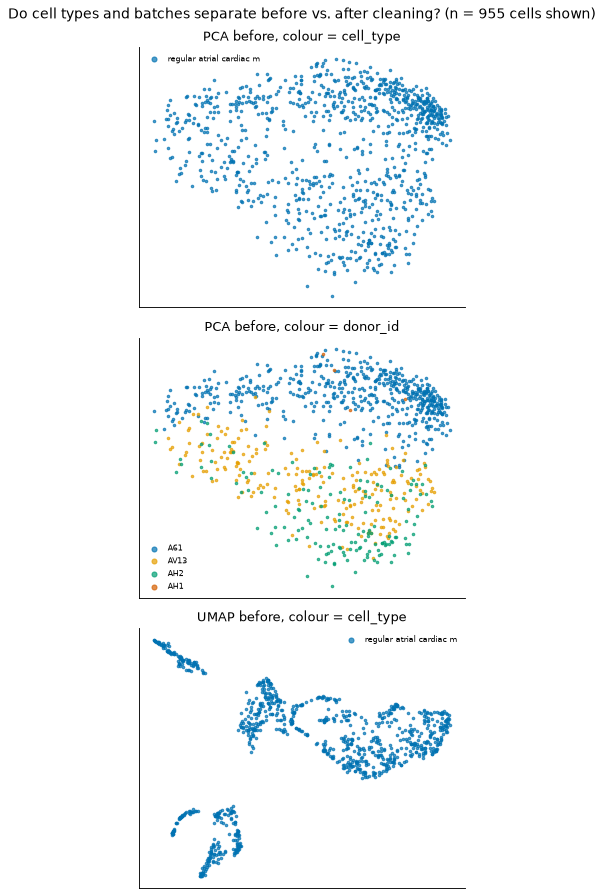
\includegraphics[width=0.85\linewidth]{../viz/embed_cxg__10x-multiome__homo-sapiens__atrioventricular-node__680029ee.png}
\caption{-   (n = 955 cells) - built from  tasks.json (raw data)}
\end{figure}
\begin{figure}[H]\centering
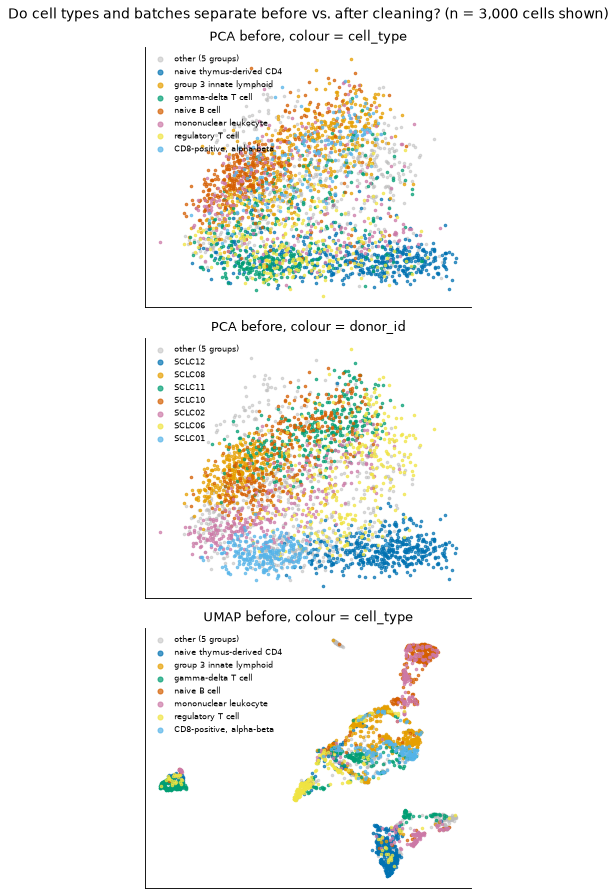
\includegraphics[width=0.85\linewidth]{../viz/embed_cxg__cel-seq2__homo-sapiens__left-main-bronchus__03da97e9.png}
\caption{-   (n = 3640 cells) - built from  tasks.json (raw data)}
\end{figure}
\begin{figure}[H]\centering
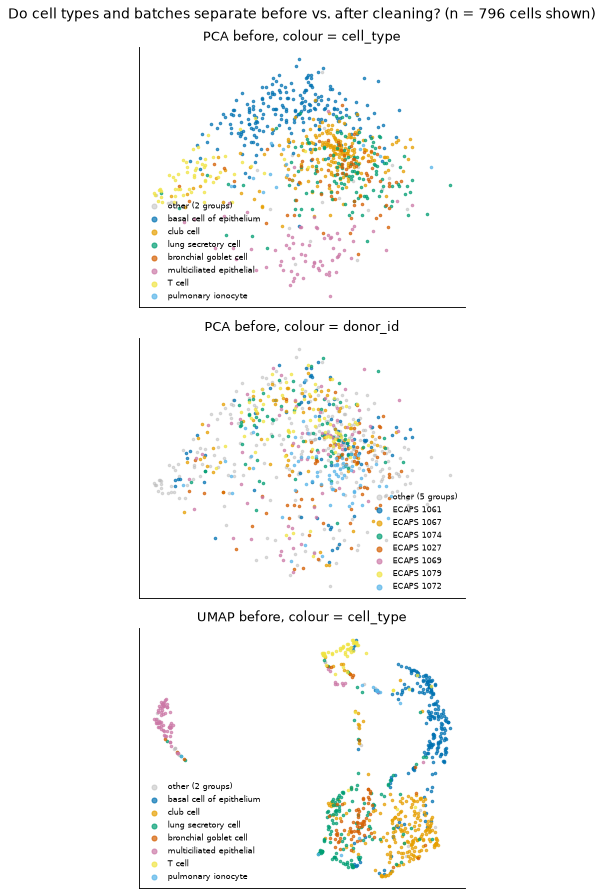
\includegraphics[width=0.85\linewidth]{../viz/embed_cxg__cel-seq__homo-sapiens__epithelium-of-main-bronchus__61d327d1.png}
\caption{-   (n = 796 cells) - built from  tasks.json (raw data)}
\end{figure}
\begin{figure}[H]\centering
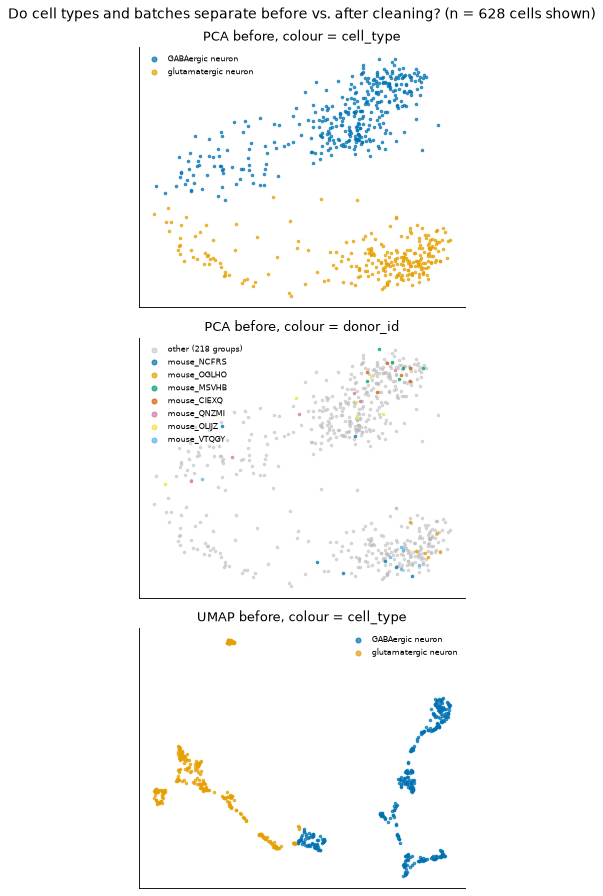
\includegraphics[width=0.85\linewidth]{../viz/embed_cxg__patch-seq__mus-musculus__primary-motor-cortex__8f98c236.png}
\caption{-   (n = 628 cells) - built from  tasks.json (raw data)}
\end{figure}
\begin{figure}[H]\centering
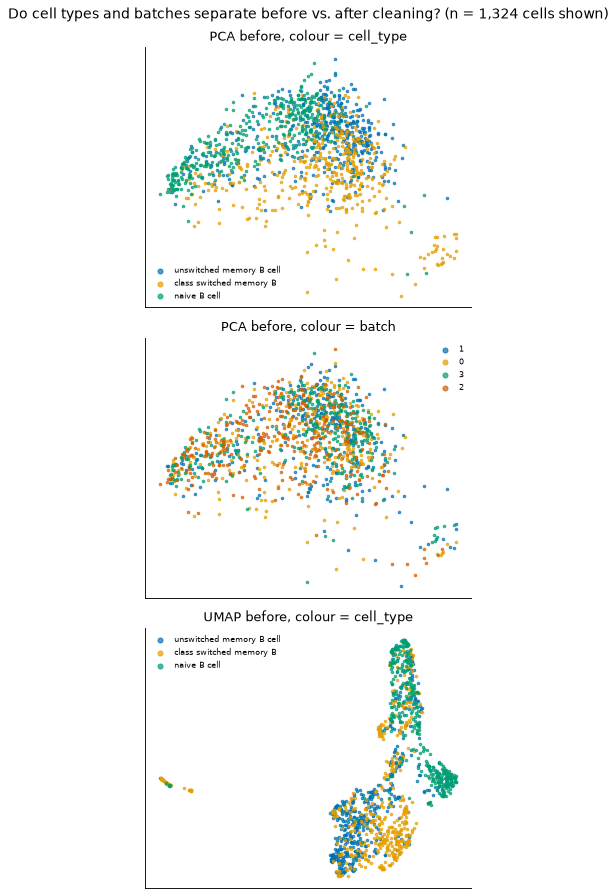
\includegraphics[width=0.85\linewidth]{../viz/embed_cxg__smart-seq2__homo-sapiens__blood__a5d95a42.png}
\caption{-   (n = 1324 cells) - built from  tasks.json (raw data)}
\end{figure}
\begin{figure}[H]\centering
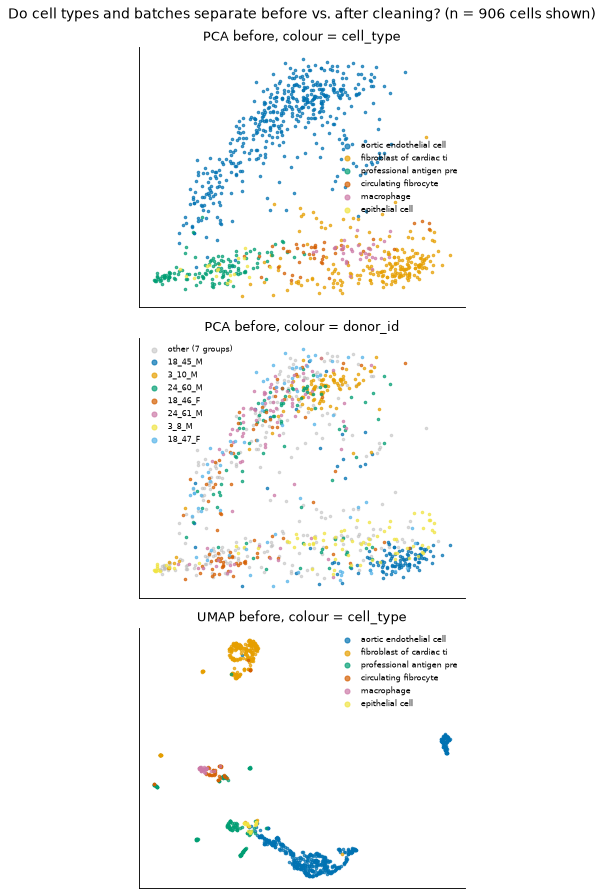
\includegraphics[width=0.85\linewidth]{../viz/embed_cxg__smart-seq2__mus-musculus__aorta__0380ddce.png}
\caption{-   (n = 906 cells) - built from  tasks.json (raw data)}
\end{figure}
\begin{figure}[H]\centering
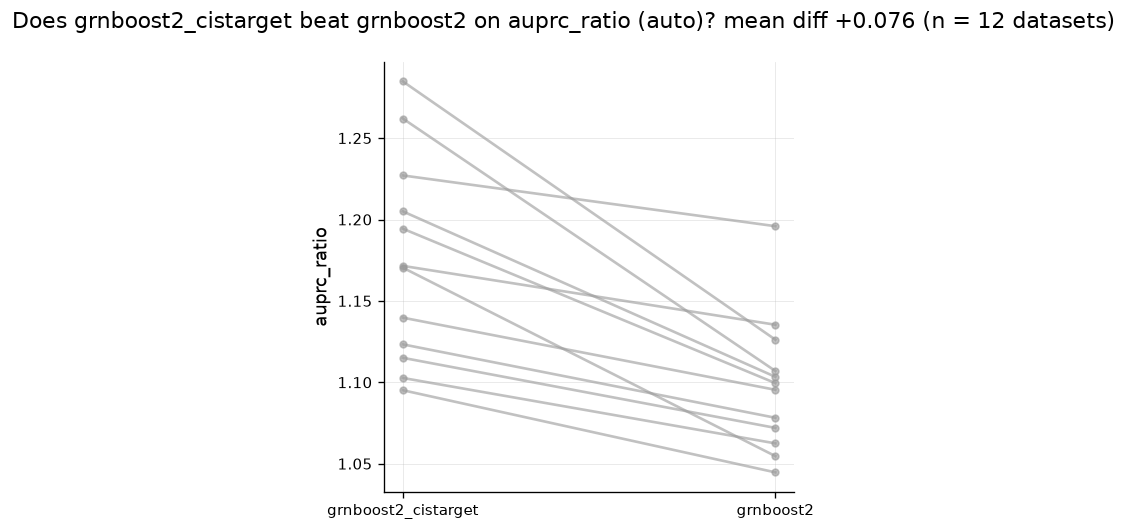
\includegraphics[width=0.85\linewidth]{../viz/lift_grnboost2_cistarget_vs_grnboost2.png}
\caption{-   (n = 12 datasets) - built from  rows/ .json (grnboost2\_cistarget vs grnboost2)}
\end{figure}
\begin{figure}[H]\centering
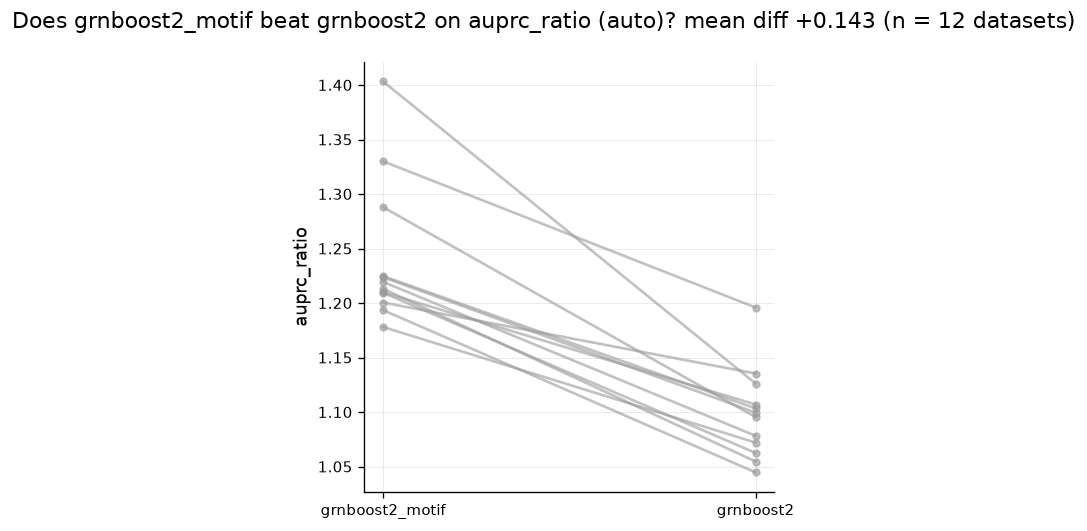
\includegraphics[width=0.85\linewidth]{../viz/lift_grnboost2_motif_vs_grnboost2.png}
\caption{-   (n = 12 datasets) - built from  rows/ .json (grnboost2\_motif vs grnboost2)}
\end{figure}
\begin{figure}[H]\centering
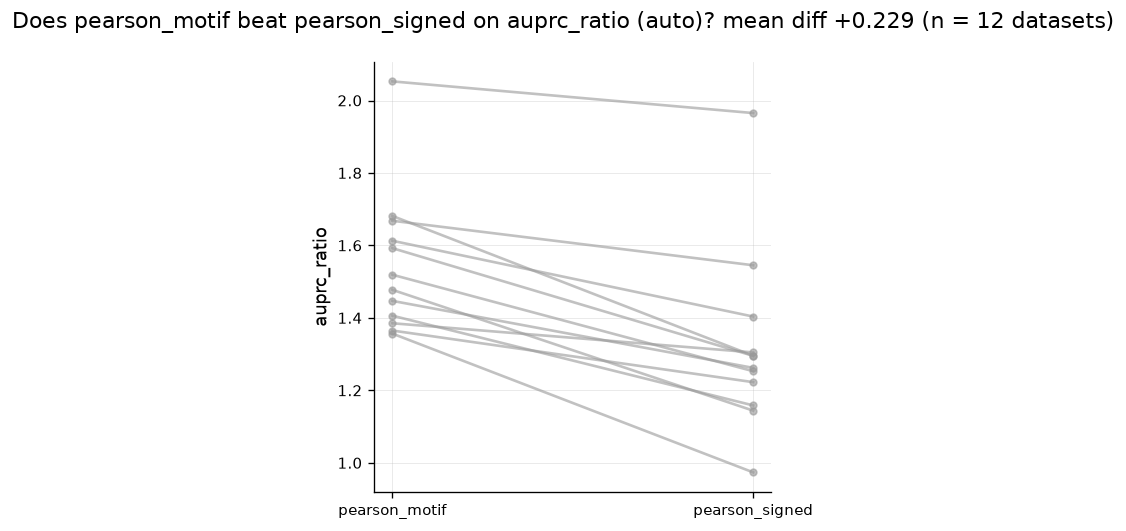
\includegraphics[width=0.85\linewidth]{../viz/lift_pearson_motif_vs_pearson_signed.png}
\caption{-   (n = 12 datasets) - built from  rows/ .json (pearson\_motif vs pearson\_signed)}
\end{figure}
\begin{figure}[H]\centering
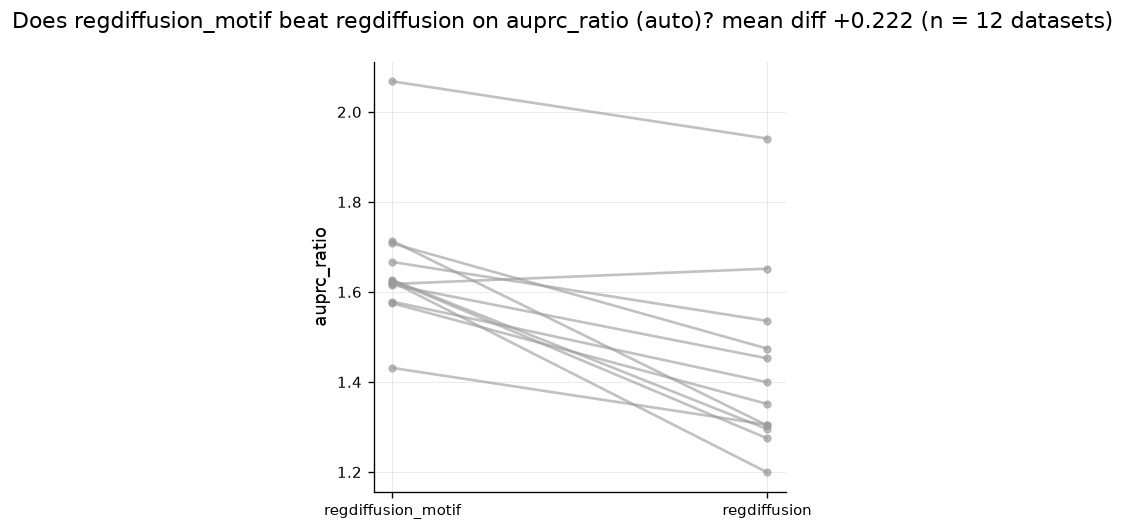
\includegraphics[width=0.85\linewidth]{../viz/lift_regdiffusion_motif_vs_regdiffusion.png}
\caption{-   (n = 12 datasets) - built from  rows/ .json (regdiffusion\_motif vs regdiffusion)}
\end{figure}
\begin{figure}[H]\centering
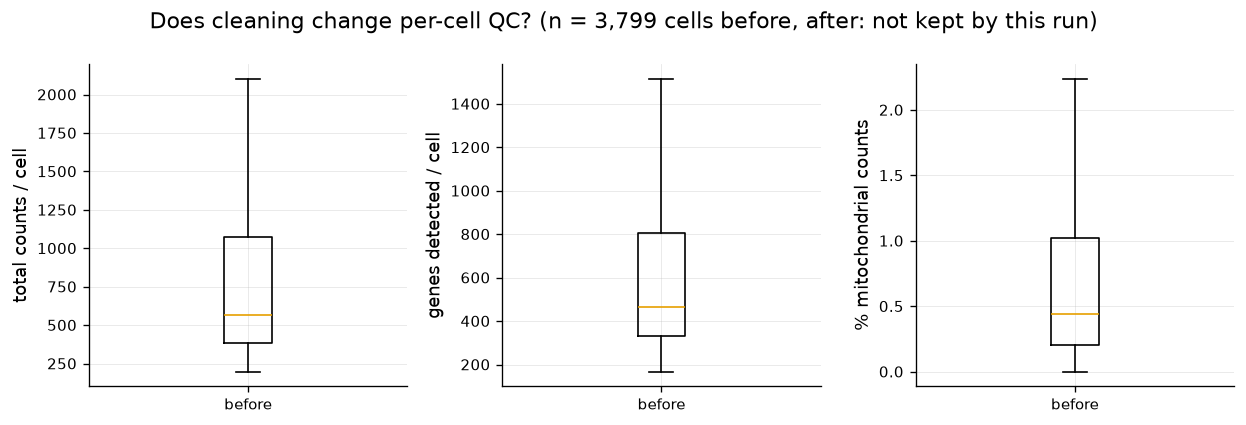
\includegraphics[width=0.85\linewidth]{../viz/qc_cxg__10x-3-v2__homo-sapiens__superior-frontal-gyrus__bdacc907.png}
\caption{-   (n = 3799 cells) - built from  tasks.json (raw data)}
\end{figure}
\begin{figure}[H]\centering
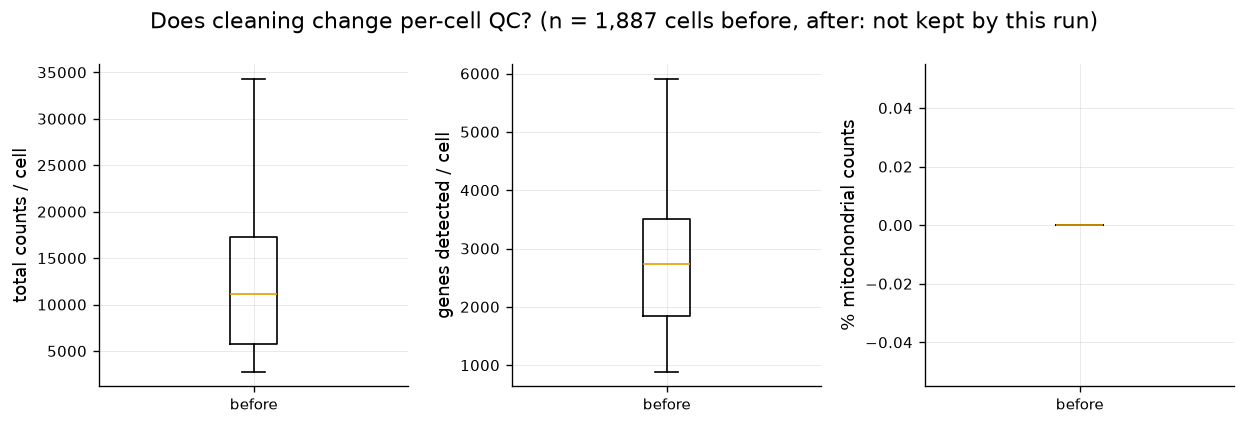
\includegraphics[width=0.85\linewidth]{../viz/qc_cxg__10x-3-v2__mus-musculus__large-intestine__de4e7a0c.png}
\caption{-   (n = 1887 cells) - built from  tasks.json (raw data)}
\end{figure}
\begin{figure}[H]\centering
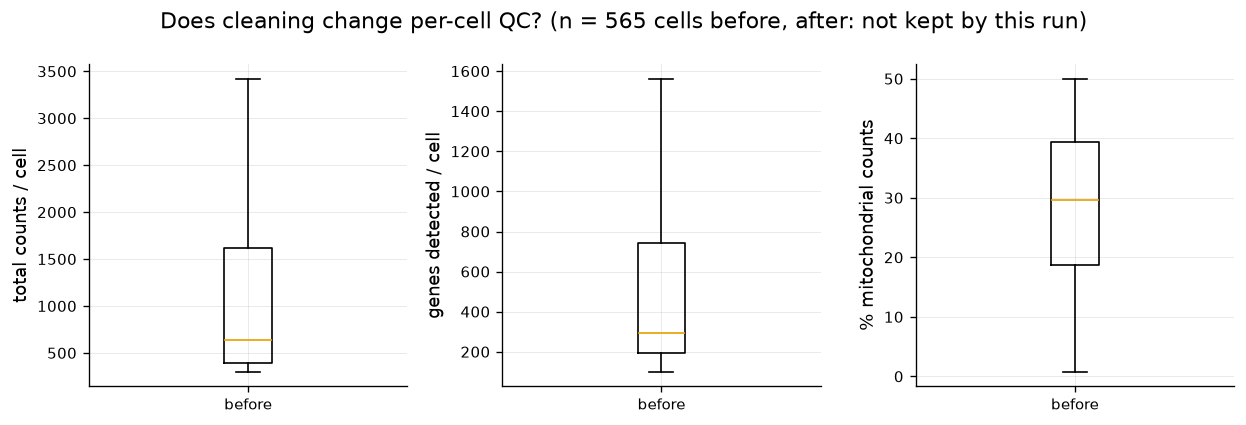
\includegraphics[width=0.85\linewidth]{../viz/qc_cxg__10x-3-v3__homo-sapiens__liver__d7476ae2.png}
\caption{-   (n = 565 cells) - built from  tasks.json (raw data)}
\end{figure}
\begin{figure}[H]\centering
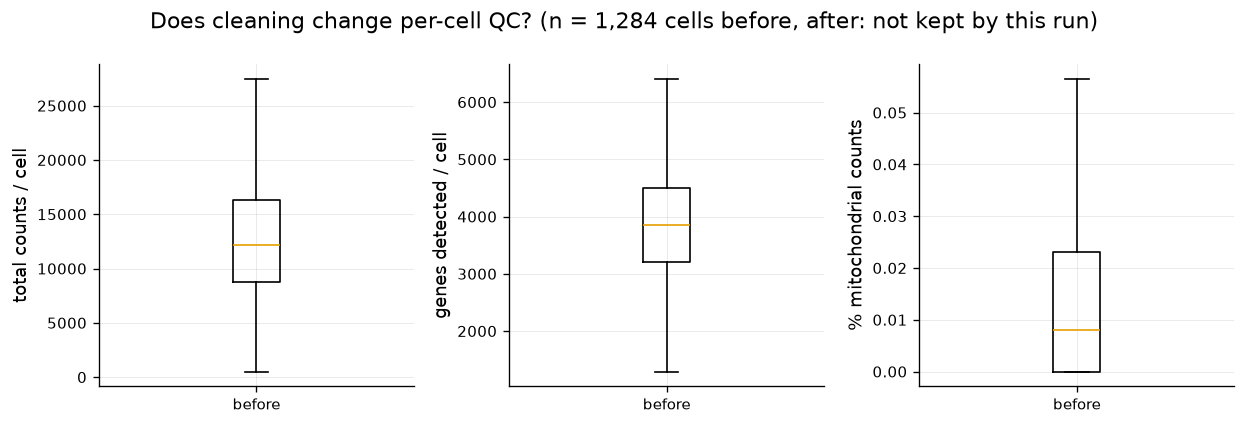
\includegraphics[width=0.85\linewidth]{../viz/qc_cxg__10x-3-v3__mus-musculus__cervical-spinal-cord__9fcd3812.png}
\caption{-   (n = 1284 cells) - built from  tasks.json (raw data)}
\end{figure}
\begin{figure}[H]\centering
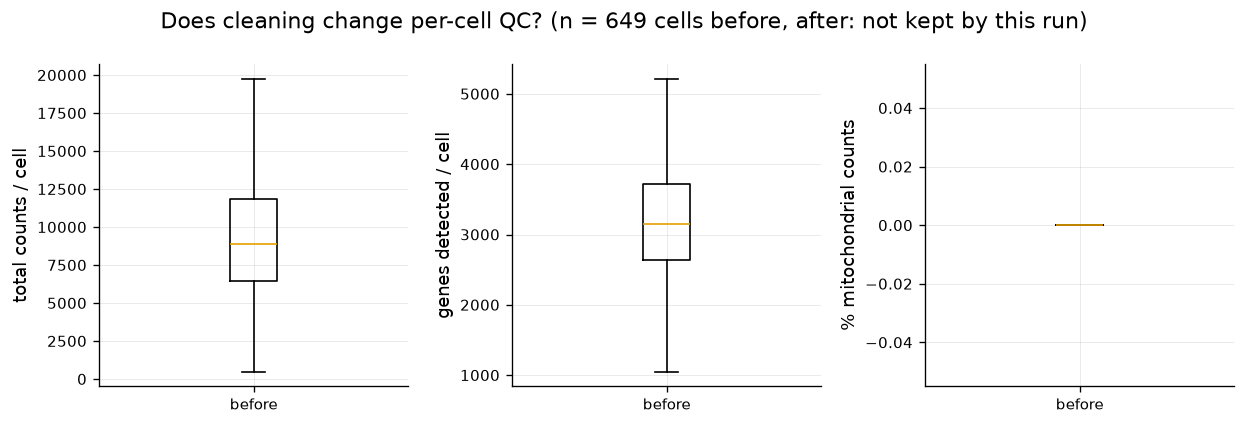
\includegraphics[width=0.85\linewidth]{../viz/qc_cxg__10x-5-v1__homo-sapiens__lung__703f00e6.png}
\caption{-   (n = 649 cells) - built from  tasks.json (raw data)}
\end{figure}
\begin{figure}[H]\centering
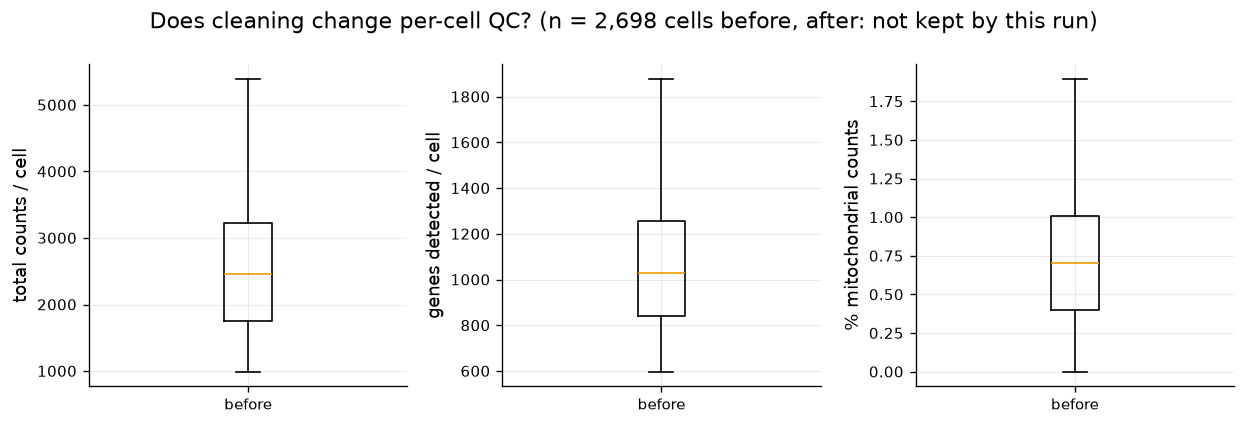
\includegraphics[width=0.85\linewidth]{../viz/qc_cxg__10x-5-v2__mus-musculus__caecum__0a1ad9d5.png}
\caption{-   (n = 2698 cells) - built from  tasks.json (raw data)}
\end{figure}
\begin{figure}[H]\centering
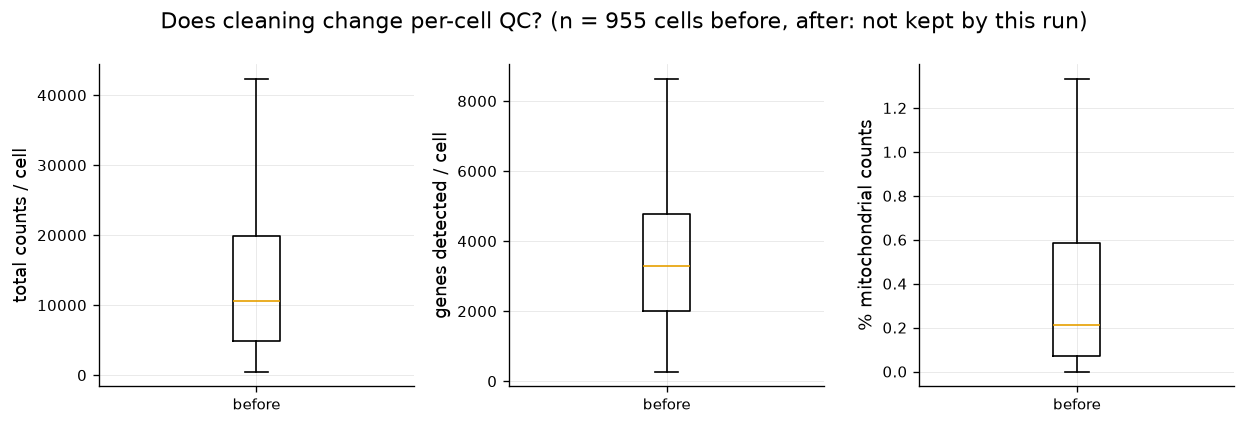
\includegraphics[width=0.85\linewidth]{../viz/qc_cxg__10x-multiome__homo-sapiens__atrioventricular-node__680029ee.png}
\caption{-   (n = 955 cells) - built from  tasks.json (raw data)}
\end{figure}
\begin{figure}[H]\centering
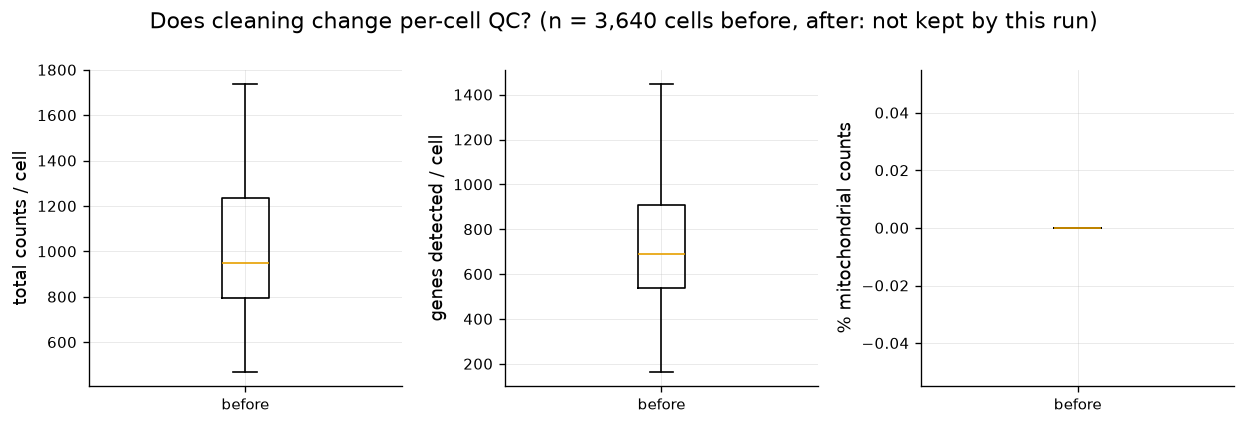
\includegraphics[width=0.85\linewidth]{../viz/qc_cxg__cel-seq2__homo-sapiens__left-main-bronchus__03da97e9.png}
\caption{-   (n = 3640 cells) - built from  tasks.json (raw data)}
\end{figure}
\begin{figure}[H]\centering
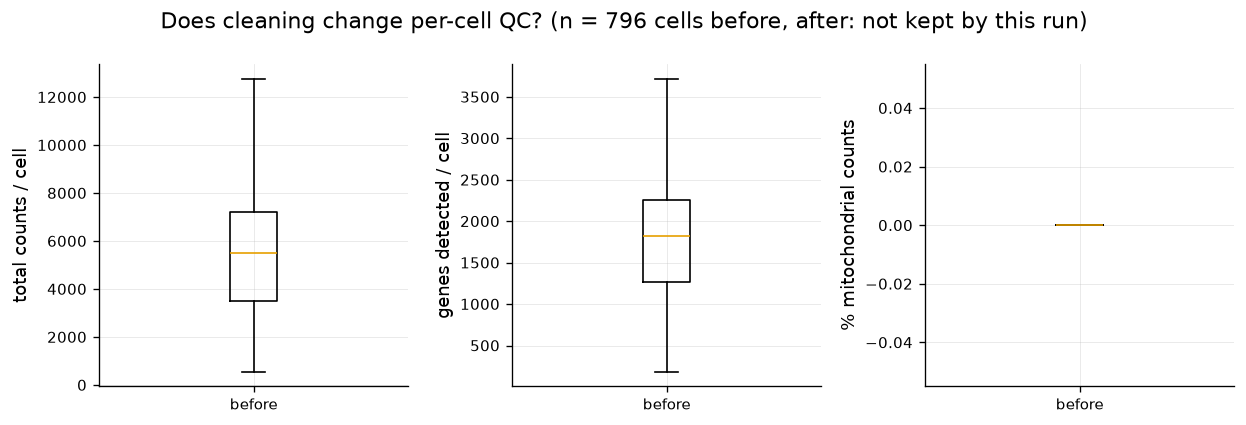
\includegraphics[width=0.85\linewidth]{../viz/qc_cxg__cel-seq__homo-sapiens__epithelium-of-main-bronchus__61d327d1.png}
\caption{-   (n = 796 cells) - built from  tasks.json (raw data)}
\end{figure}
\begin{figure}[H]\centering
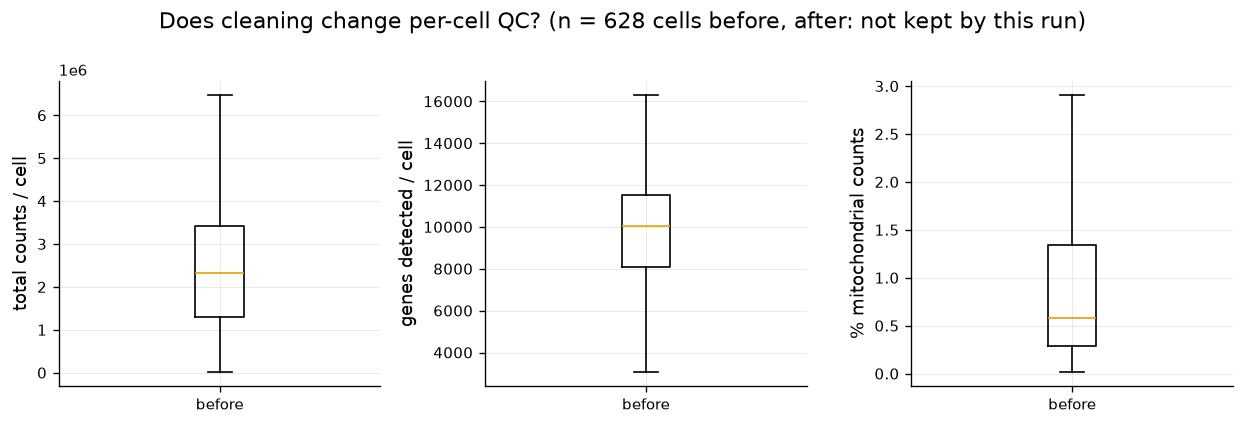
\includegraphics[width=0.85\linewidth]{../viz/qc_cxg__patch-seq__mus-musculus__primary-motor-cortex__8f98c236.png}
\caption{-   (n = 628 cells) - built from  tasks.json (raw data)}
\end{figure}
\begin{figure}[H]\centering
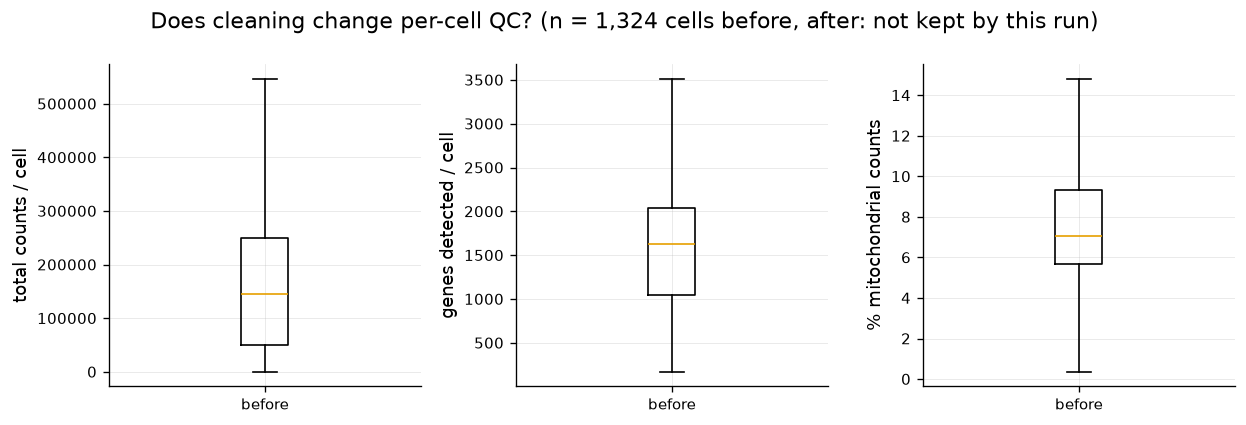
\includegraphics[width=0.85\linewidth]{../viz/qc_cxg__smart-seq2__homo-sapiens__blood__a5d95a42.png}
\caption{-   (n = 1324 cells) - built from  tasks.json (raw data)}
\end{figure}
\begin{figure}[H]\centering
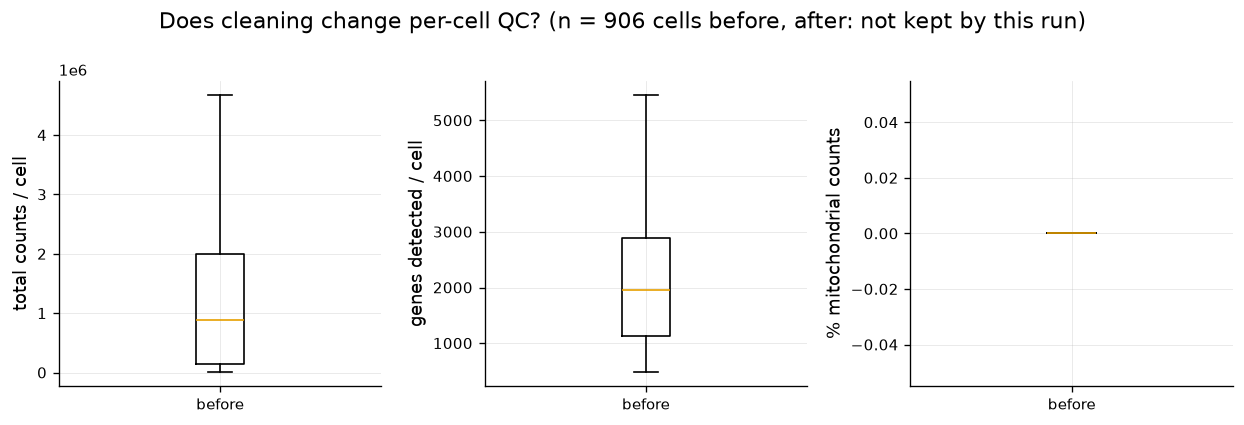
\includegraphics[width=0.85\linewidth]{../viz/qc_cxg__smart-seq2__mus-musculus__aorta__0380ddce.png}
\caption{-   (n = 906 cells) - built from  tasks.json (raw data)}
\end{figure}
\begin{figure}[H]\centering
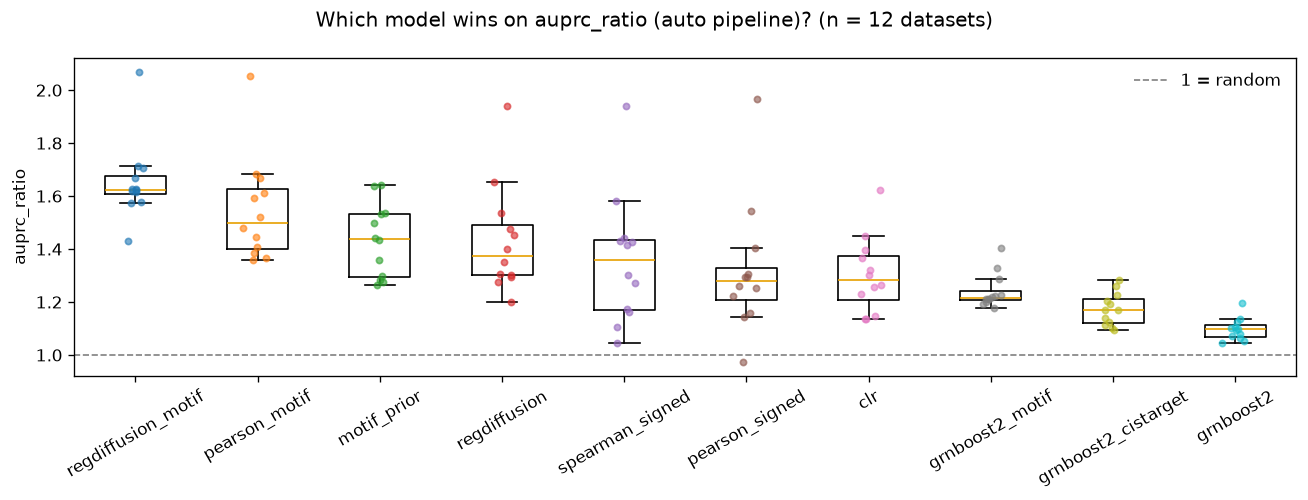
\includegraphics[width=0.85\linewidth]{../viz/scores_auprc_ratio_auto.png}
\caption{-   (n = 12 datasets) - built from  rows/ .json (auto/auprc\_ratio)}
\end{figure}
\begin{figure}[H]\centering
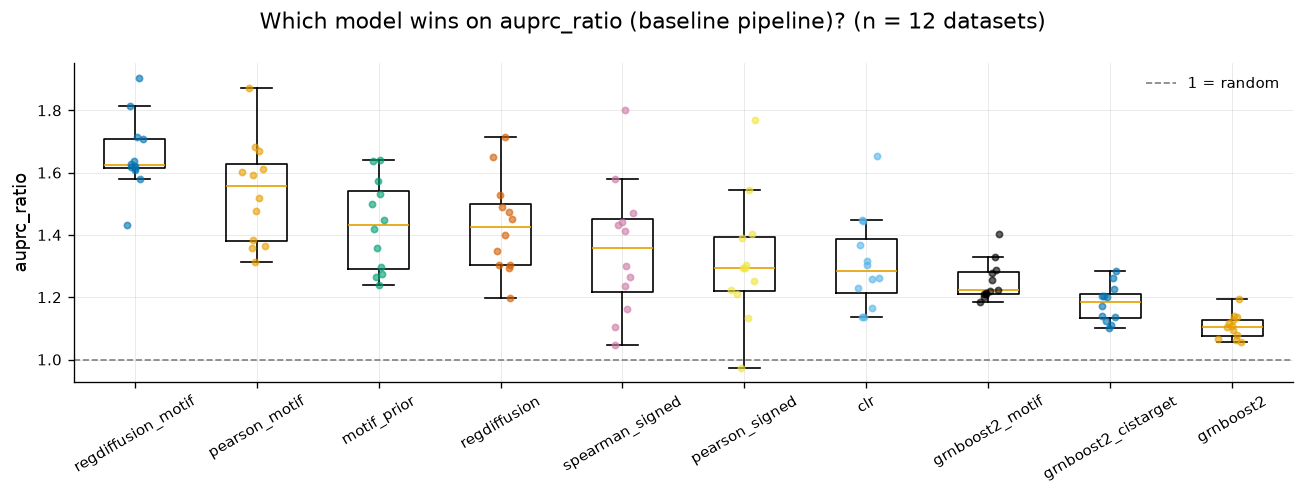
\includegraphics[width=0.85\linewidth]{../viz/scores_auprc_ratio_baseline.png}
\caption{-   (n = 12 datasets) - built from  rows/ .json (baseline/auprc\_ratio)}
\end{figure}
\begin{figure}[H]\centering
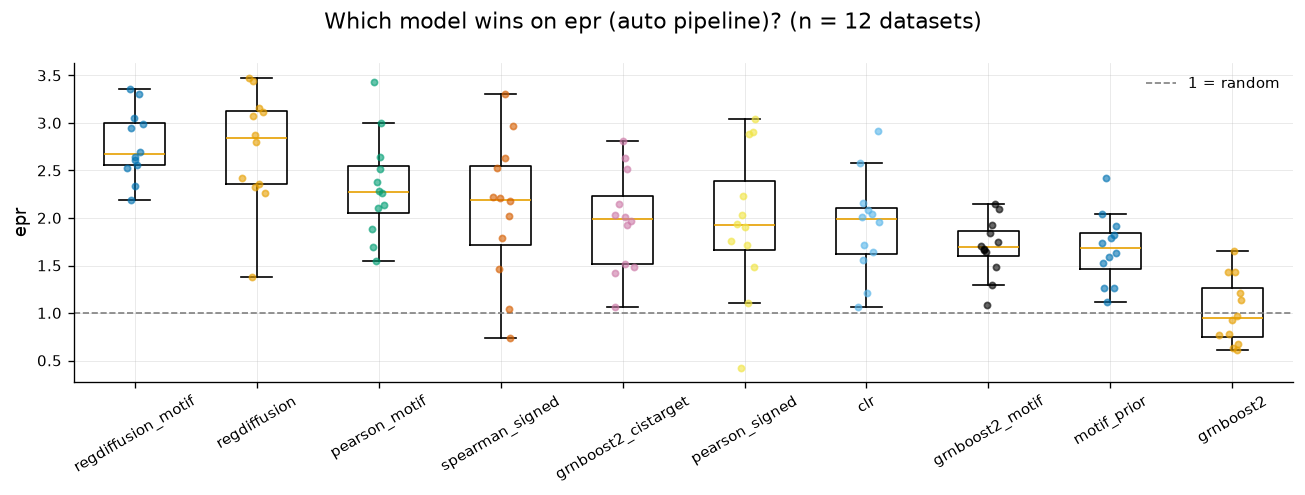
\includegraphics[width=0.85\linewidth]{../viz/scores_epr_auto.png}
\caption{-   (n = 12 datasets) - built from  rows/ .json (auto/epr)}
\end{figure}
\begin{figure}[H]\centering
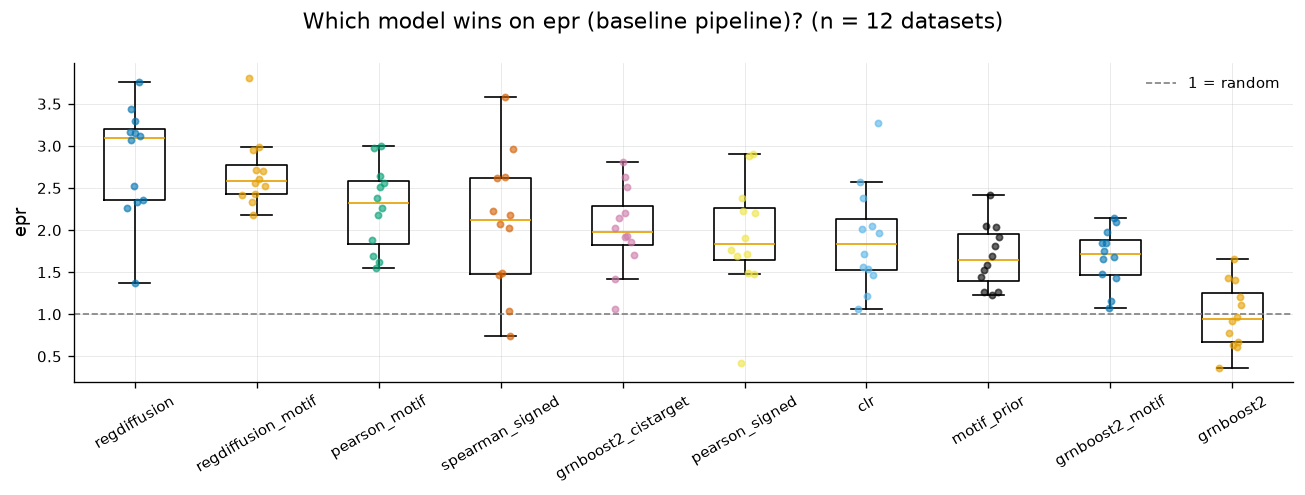
\includegraphics[width=0.85\linewidth]{../viz/scores_epr_baseline.png}
\caption{-   (n = 12 datasets) - built from  rows/ .json (baseline/epr)}
\end{figure}

\section{Limitations}
\begin{itemize}
\item Exploratory experiment: results need a confirmatory rerun before a headline claim.
\item Recorded deviation: scikit-image was not installed, so wherever the plan chose scrublet (rows show doublets: scrublet) doublet calling most likely fell back to the heuristic caller with a warning (found 2026-09-25 while setting up the repo; not yet checked in the run manifests).
\item The run did not record which doublet caller ran (rows predate the fallback record).
\end{itemize}

\end{document}
